\subsection{The Flat-Sky approximation and Extended Limber Approximation}
The baseline measurement for many cosmic shear studies has focused on the two-point shear correlation function between two tomographic bins $ij$ \citep[for more details see][and references therein]{bartelmann/schneider:2001}, given by
\be
\xi_\pm^{ij}(\theta) = \frac{1}{2\pi}\int \d\ell \,\ell \,P^{ij}_\kappa(\ell) \, J_{0,4}(\ell \theta) \, , 
\label{eqn:xiGG}
\ee
where $J_{0,4} (\ell \theta)$ is the zeroth (for $\xi_+$) or fourth (for $\xi_- $) order Bessel function of the first kind and $P_\kappa(\ell)$ is the convergence power spectrum at angular wave number $\ell$ which can be related to the underlying matter power spectrum $P_\delta$, using a Limber approximation as,
\be 
P^{ij}_\kappa(\ell) = T_l \int_0^{\chi_{\rm H}} \d \chi \, \frac{q_i(\chi)q_j(\chi)}{[f_K(\chi)]^2} \, P_\delta \left( \frac{\nu}{f_K(\chi)},\chi \right).
\label{eqn:Pkappa} 
\ee
Here $f_K(\chi)$ is the comoving angular diameter distance out to comoving radial distance $\chi$ and $\chi_{\rm H}$ is the comoving horizon distance.  The lensing efficiency function $q(\chi)$ is given in equation (5) of \citet{hildebrandt/etal:2016}.   \citet{kitching/etal:2016} show that the pre-factor $T_\ell$ is given by
\be
T_\ell = \frac{(\ell+2)(\ell+1)\ell(\ell-1)}{(\ell + 0.5)^4} \, .
\label{eqn:Tl}
\ee
When a survey is sufficiently small, a flat-sky approximation can be made reducing $T_\ell \approx 1$.  The value of $\nu$ depends on whether a baseline Limber approximation, or the more accurate extended Limber approximation of \citet{loverde/afshordi:2008} is used.  In the analysis of \citet{kitching/etal:2016} it is not fully clear which combinations of  $T_\ell$ and $\nu$ are considered, so we review them all as summarised in Table~\ref{tab:Tl_nu}, also highlighting which combinations were used in recent cosmic shear analyses.

 \begin{table}[htb]
\label{tab:Tl_nu}
\begin{center}
\begin{tabular}{ | l | c | c  | c |}
\hline
Case & $T_\ell$ & $\nu$ & Used in \\ \hline
\citet{kitching/etal:2016} `Standard' & $1$ & $\ell$ & pre-2014 CFHTLenS papers \\
Baseline Limber Flat Sky &  $\ell^4 / (\ell + 0.5)^4$ & $\ell$ & \\
Baseline Limber Spherical & equation~\ref{eqn:Tl} & $\ell$ & \\
Extended Limber Flat Sky & $\ell^4 / (\ell + 0.5)^4$ & $\ell + 0.5$ & \\
Extended Limber Spherical & equation~\ref{eqn:Tl}& $\ell + 0.5$  & \\
Extended `Standard' & $1$ & $\ell + 0.5$ & \citet{joudaki/etal:2016} \&  \\
  & & & \citet{hildebrandt/etal:2016}$^*$\\\hline
 \end{tabular}
 \end{center}
 \caption{Variations on the different approximations that can be made when calculating the convergence power spectrum $P_\kappa(\ell)$ (equation~\ref{eqn:Pkappa}), using a Limber approximation.  $^*$We confirm that there is a typographical error in equation 4 of \citet{hildebrandt/etal:2016} which does not include the extra term of `$+0.5$' in $\nu$ that was incorporated in the cosmological analysis.}  
 \end{table}

{\bf TBD: add figures of $P_\kappa$ and $\xi_\pm$ for all these combinations showing that they make absolutely no difference.}
 
 \begin{figure}
 \begin{center}
 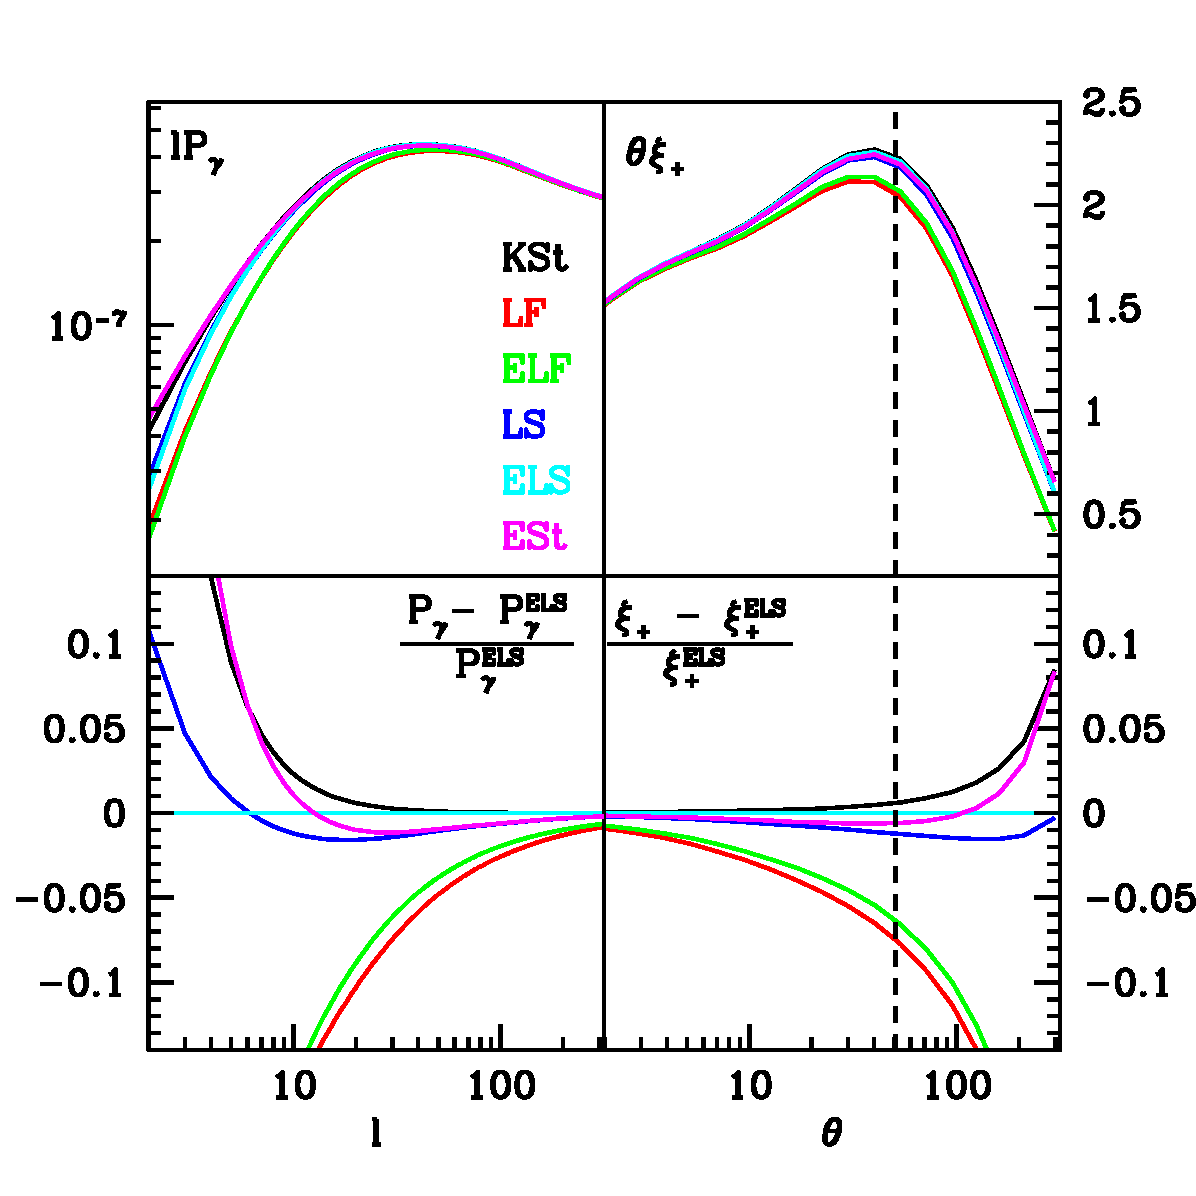
\includegraphics[width=0.5\textwidth]{figures/Cl_xi_comp.pdf}
 \label{fig:Cl_xi}
 \caption{\emph{Top:} Theoretical models of the $\kappa$ power spectrum (\emph{left}) and shear correlation function $\xi_+$ (\emph{right})for the different approximations discussed in \citet{kitching/etal:2016}. \emph{Bottom:} Deviations with respect to the full treatment (LSH).}
 \end{center}
 \end{figure}
 
 \subsection{Cosmic shear without the Limber Approximation}
In collecting our comments on \citet{kitching/etal:2016} we contacted colleagues who had previously tested the impact of the Limber approximation on cosmic shear studies by comparing a Limber approximated cosmic shear power spectrum with an exact calculation.  The majority of these analyses, carried out many years ago, remained unpublished as no significant deviation was found.  One notable exception, however, is \citet{giannantonio/etal:2012} who find that for a cosmic shear power spectrum, the extended Limber approximation is consistent with the exact calculation for $\ell>5$, with any differences well within cosmic-variance errors for a Euclid-like survey\footnote{\citet{kitching/etal:2016} comment on this result, but indicate that it is in error owing to the application of a fixed low-$\ell$ limit.  \citet{giannantonio/etal:2012} however state that this limit is only applied in a positive curvature case.}.  We therefore argue that the assertion by \citet{kitching/etal:2016} that the majority of cosmic shear data analyses to date have made an `axiomatic assumption (i.e. an unquestioned and untested assumption at the beginning of the analysis)'  is unwarranted.  Not only is there published work that has questioned and tested the Limber approximation for cosmic shear studies, individual teams have also verified this result internally.    

Given the insignificant effect of using the Limber approximation found by various groups, the ability to calculate an exact non-Limber solution has unfortunately not been maintained in theoretical code over the years.  Instead these codes have evolved to account for important approximations such as the impact of baryon feedback on the matter power spectrum and non-zero neutrino masses \citep[see for example][]{joudaki/etal:2016, mead/etal:2016}.    We are therefore unable to readily determine non-Limber theoretical calculations for the shear-correlation function to directly compare with the results of \citet{kitching/etal:2016}.   Instead we refer the reader to Figure 3 of \citet{giannantonio/etal:2012} to draw their own conclusions.



 
 
 
 
 
 
 